\chapter{Background} \label{chap:background}
In the frame of this thesis, knowledge about \acrshort{cnn} and \acrshort{fpga} is required. The purpose of this chapter is then to detail all these background information.

First, Secion \ref{sec:cnn} develops the theory behind \acrshort{cnn}. We explore how such model can be constructed, what are the state-of-the-models and how can we train it.

Finally, Section \ref{sec:fpga} explains what is a \acrshort{fpga} and what are its main components. We also detail the \acrshort{fpga} design flow.
% Cnn
\section{Convolutional Neural Network} \label{sec:cnn}
\acrshort{cnn} is a type of \acrshort{nn} specialized in analyzing visual imagery and natural language processing. \acrshort{cnn}s are feedforward, sparsely connected \acrshort{nn}s, and structured as a pipeline of layers \cite{abdelouahab_accelerating_2018}. It showed superior performances in different competitions related to Computer Vision and Image Processing \cite{khan_survey_2020}. Nowadays, \acrshort{cnn}s are used in character and gesture recognition, video classification, face detection, etc \cite{shawahna_fpga-based_2019}. This section aims at investigating the different aspects of a \acrshort{cnn}.

First, the building blocks of a CNN are developed in Section \ref{subsec:layer} starting from its basic element, the \textit{perceptron}. Then, we describe how to use multiple perceptrons to build layers that can perform complex functions. Finally, we detail the other types of layers required to improve the efficiency of the model, such as the pooling layer.

Then, Section \ref{subsec:models} describes how to effectively combine these layers with a focus on the state-of-the-art networks like AlexNet, VGG16, ResNet, and MobileNetV2.

Finally, Section \ref{subsec:train} focuses on the training of \acrshort{cnn}. We briefly explain the back-propagation algorithm, which consists of a forward-propagation and a back-propagation.
%
%
\subsection{Structure of a CNN} \label{subsec:layer}
%
\acrshort{cnn} is a pipeline of layers that can be stacked to form a network \cite{abdelouahab_accelerating_2018}. A layer is a high-level building block, which consists of a set of operations, weights, and non-linear functions. The output of one layer can be used as input of the next layer or as the final output of the network. 

This section first introduces the simplest building element of a \acrshort{cnn}: the perceptron. We describe its different components and notably its activation function. Then, we can use this element to build more complex layers such as the fully connected and convolutional layer. Finally, we present the pooling layer which is used to reduce the spatial dimensions of the output of the previous layer.
%
%
\subsection{Perceptron} \label{subs:perceptron}
The perceptron was developed in 1957 by \textcite{rosenblatt_perceptron_1958}. The idea is to compare the computational model to a human brain which is composed of a large number of units called neurons. A neuron receives an information and when its threshold is reached (we say the neuron fires), this information is released and transmitted to other neurons \cite{rosenblatt_perceptron_1958, matteucci_artificial_2019}.

\begin{figure}
    \centering
    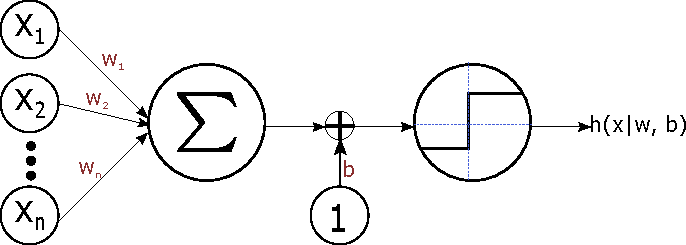
\includegraphics[width=0.8\textwidth]{perceptron.pdf}
    \caption{The Perceptron}
    \label{fig:perceptron}
\end{figure}
%
This neuron in a human brain corresponds to a perceptron in the computational model. It is composed of $n_{in}$ inputs $\boldsymbol{x} = \{ x_1, ... x_{n_{in}} \}$, $n_{in}$ weights $\boldsymbol{w}$ and a bias $b$. Figure \ref{fig:perceptron} illustrates the working principle of a perceptron. When a perceptron received an input vector $\boldsymbol{x}$, a weighted sum of this vector is performed. If its result is higher than the threshold (controlled by $b$), the perceptron is \textquote{activated} and its output becomes a non-zero value.
Equation \ref{eq:perceptron} represents the mathematical formula of the perceptron where $h$ is the activation function of the formula developed in Equation \ref{eq:step} \cite{matteucci_artificial_2019}.
%
\begin{equation}
    h ( \boldsymbol{x} | \boldsymbol{w}, b) = h \left( \sum^{n_{in}}_{i=1} x_i \cdot w_i + b \right) = h \left( \boldsymbol{w}^{T} \cdot \boldsymbol{x} + b \right)
    \label{eq:perceptron}
\end{equation}
%
\begin{equation}
    h ( \boldsymbol{w}^{T} \cdot \boldsymbol{x} + b) = \begin{cases} 1, & \mbox{if } \boldsymbol{w}^{T} \cdot \boldsymbol{x} + b > 0 \\ 0, & \mbox{Otherwise} \end{cases}
    \label{eq:step}
\end{equation}

As the perceptron performs a weighted sum, those weights can be learned to perform a task of interest. However, this model is limited by the functions it can achieve. In Section \ref{subs:fcl}, we discover how we can use multiple perceptrons to create a \textbf{fully-connected layer} to learn more complex functions.

%
\subsection{Activation of a perceptron} \label{subs:acti}
In order to decide if a perceptron is activated or not (if its threshold is reached), an activation function needs to be defined. However, to use this function in a \acrshort{dl} model and be able to apply the back-propagation algorithm (will be further detailed in Section \ref{sec:train}), this function needs to be differentiable \cite{lecun_backpropagation_1989}. Indeed, during the optimization of the network, the gradient of the activation function is computed. Therefore, Equation \ref{eq:step} cannot be used as the activation function because of its zero gradient and the learning does not converge.  Various activation functions have been proposed with different properties, as illustrated in Figure \ref{fig:acti}. According to \textcite{khan_survey_2020}, the choice of an appropriate activation function can accelerate the learning phase and some activations decrease the computational complexity \cite{krizhevsky_imagenet_2012}.
%
\begin{figure}
    \centering
    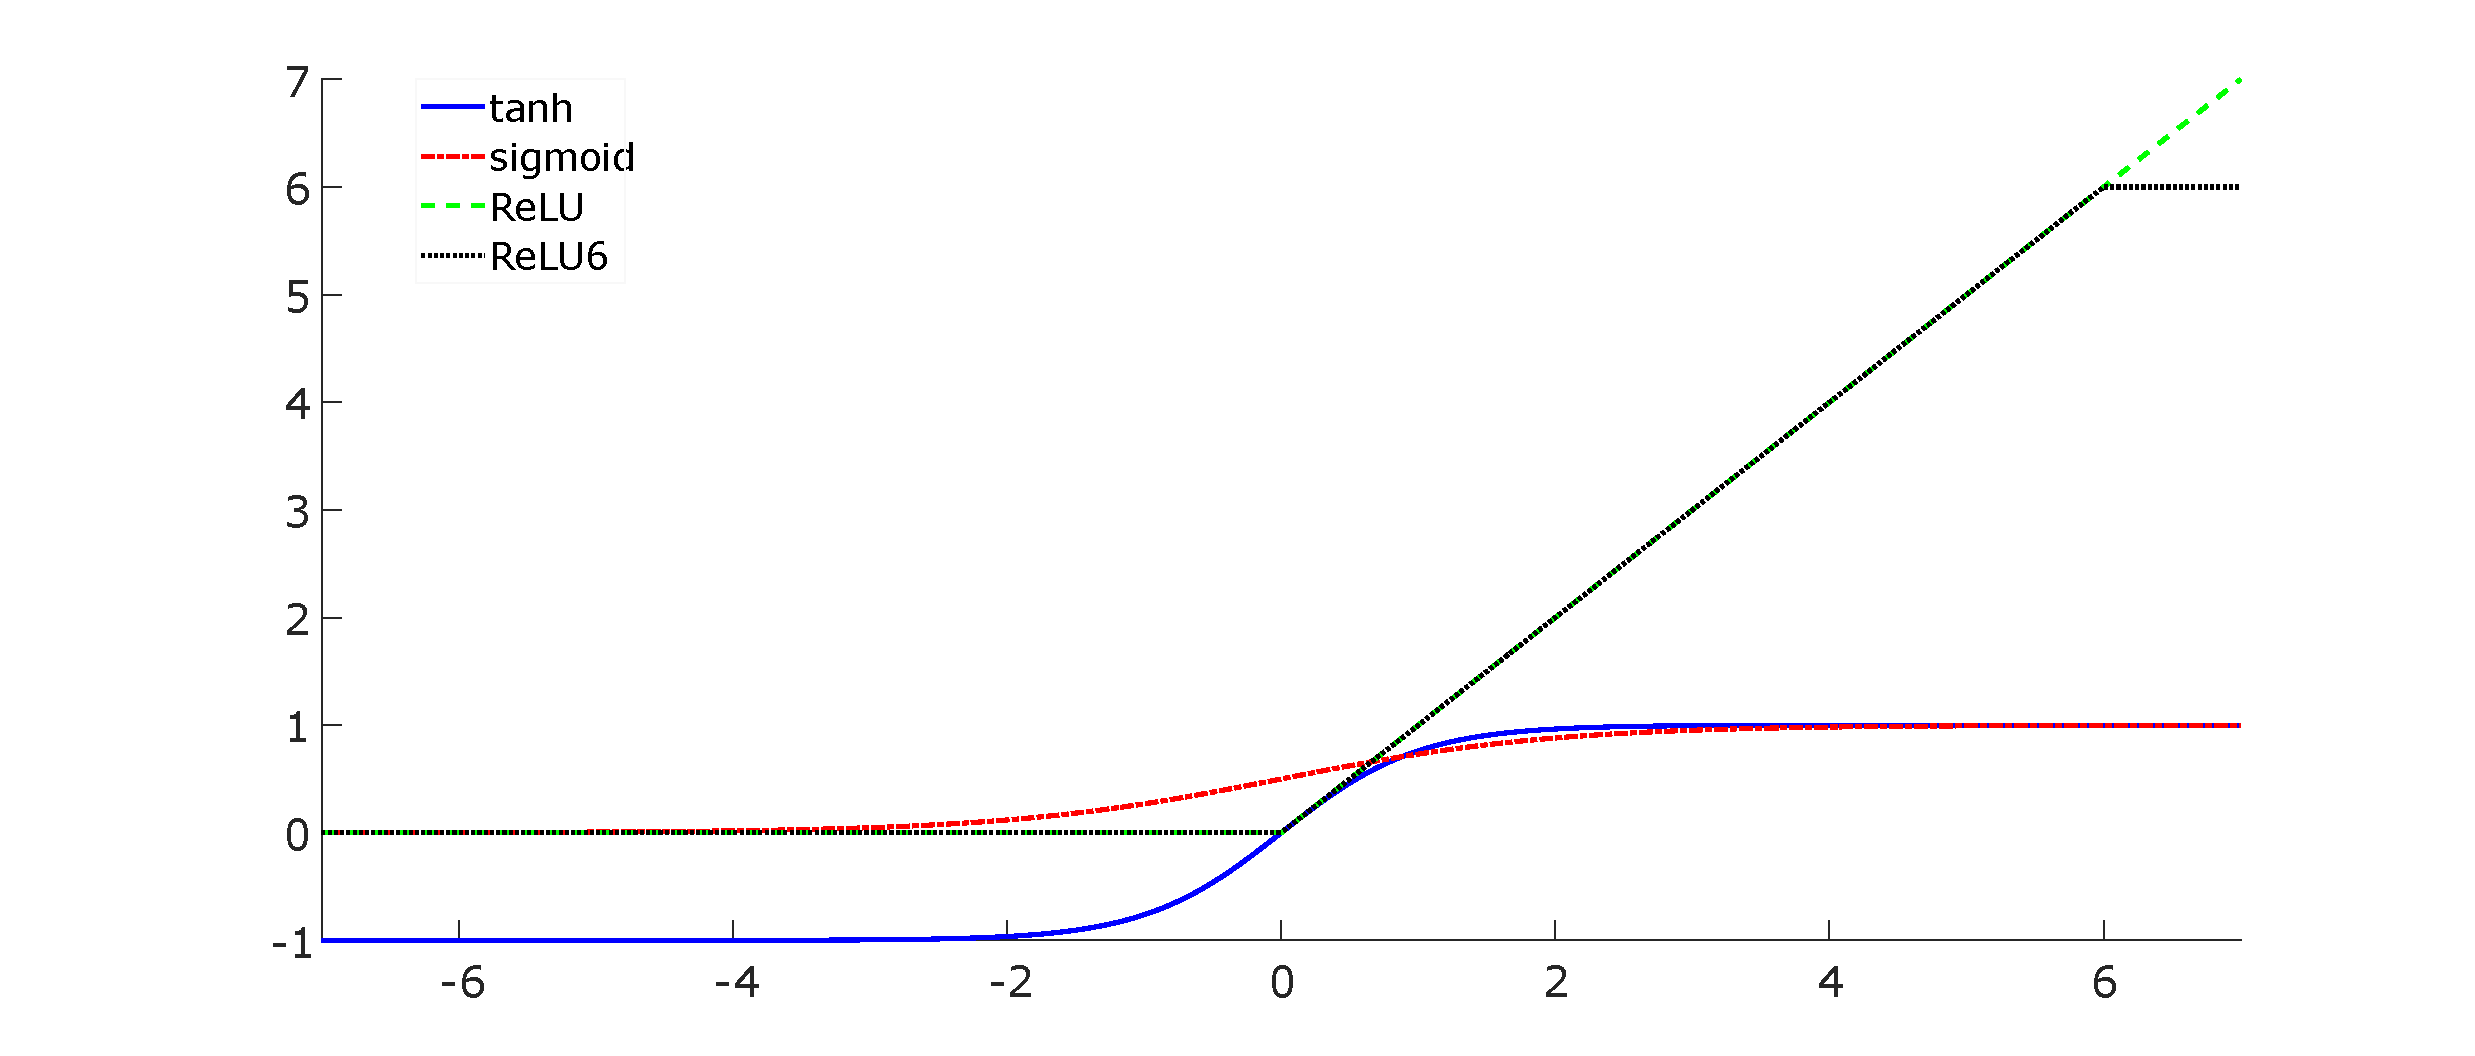
\includegraphics[width=\textwidth]{actifun.pdf}
    \caption{Activation functions}
    \label{fig:acti}
\end{figure}
%
\subsubsection{Sigmoid and Hyperbolic Tangent (Tanh)}
$Sigmoid$ and $Tanh$ are both smooth functions that can be described by equations \eqref{eq:sigmoid} and \eqref{eq:tanh} \cite{krizhevsky_imagenet_2012}.
%
\begin{equation}
    h(x) = \frac{1}{1 + e^{-x}}
    \label{eq:sigmoid}
\end{equation}
%
\begin{equation}
    h(x) = \frac{e^{x} - e^{-x}}{e^{x} + e^{-x}}
    \label{eq:tanh}
\end{equation}
%
These two activation functions can be seen in Figure \ref{fig:acti}. They both limith the $\mathbb{R}$ domain into a narrower domain, $[0, 1]$ for $Sigmoid$, and $[-1, 1]$ for the $Tanh$. However, they also saturate at the asymptotes, which means that often their gradient is close to 0 \cite{glorot_understanding_2010}. As the back-propagation algorithm (see Section \ref{sec:train}) requires gradient multiplication, gradient far away from the output vanishes (close to 0) and deep models do not learn: it is the \textbf{vanishing gradient problem} \cite{goodfellow_deep_2016, khan_survey_2020, maas_rectier_2014}.
%
\subsubsection{ReLU}
In order to overcome this vanishing gradient problem, the Rectified Linear Unit (ReLU) which is defined by Equation \eqref{eq:relu} has been developed by \textcite{krizhevsky_imagenet_2012}.
%
\begin{equation}
    h(x) = max(0, x)
    \label{eq:relu}
\end{equation}
%
This function increases the learning and computational speed compared to the $Tanh$ and $Sigmoid$ functions and improves the propagation gradient efficiency (to avoid vanishing or exploding gradient) \cite{maas_rectier_2014, abdelouahab_accelerating_2018}. However, in this function, some perceptrons can become inactive which means that their output is zero for all input. It is called the \textbf{dying neuron problem} which decreases the model capacity \cite{matteucci_artificial_2019}. A solution would be to discard these inactive neurons by transforming the ReLU into a leaky ReLU \cite{maas_rectier_2014} activation function for example.

We can also use the dying neuron property to learn sparse features earlier. It has been done by \textcite{krizhevsky_convolutional_nodate} by setting an upper bound to the ReLU output. For example, in the work, the output is described by Equation \eqref{eq:relu6} and this activation function is called ReLU6 because the range is limited to $[0, 6]$. ReLU has also the advantage to be designed for fixed-point operations and quantization approaches (which will be more described in Section \ref{subsec:mdopti}), instead of floating-point operations. Indeed, floating-point operations, especially on \acrshort{fpga}, are less efficient in terms of hardware utilization and power consumption \cite{david_hardware_2007}. It means that if for example the output $ \in [0, 6]$, the number of bits for the integer part can be limited to 3 bits. The accuracy of the model can thus be increased by assigning the other available bits to the decimal part. For example, ReLU6 is used in model that aims mobile and embedded platforms like MobileNet \cite{howard_mobilenets_2017}. In this work, the ReLU6 activation function is used.
%
\begin{equation}
    h(x) = max(0, x, 6)
    \label{eq:relu6}
\end{equation}

%
\subsection{Fully Connected layer} \label{subs:fcl}
The perceptron of section \ref{subs:perceptron} can be considered as a linear classifier for which the decision boundary is the hyperplane, as seen in equation \eqref{eq:linearclassifer}.
%
\begin{equation}
    b + w_1 \cdot x_1 + ... + w_{n_{in}} \cdot x_{n_{in}} = 0
    \label{eq:linearclassifer}
\end{equation}
%
We can understand why the perceptron is limited because it has only a linear decision boundary. For example, we can implement the AND and OR Boolean functions using a perceptron, but it is impossible to learn the XOR function. To have a non-linear model, we must use a topology of perceptrons. The topology is composed of layers of perceptrons, where each layer, in the case of a \acrshort{cnn}, is called a \textbf{fully-connected layer}. We can see an example in figure \ref{fig:fcn}.
%
\begin{figure}
    \centering
    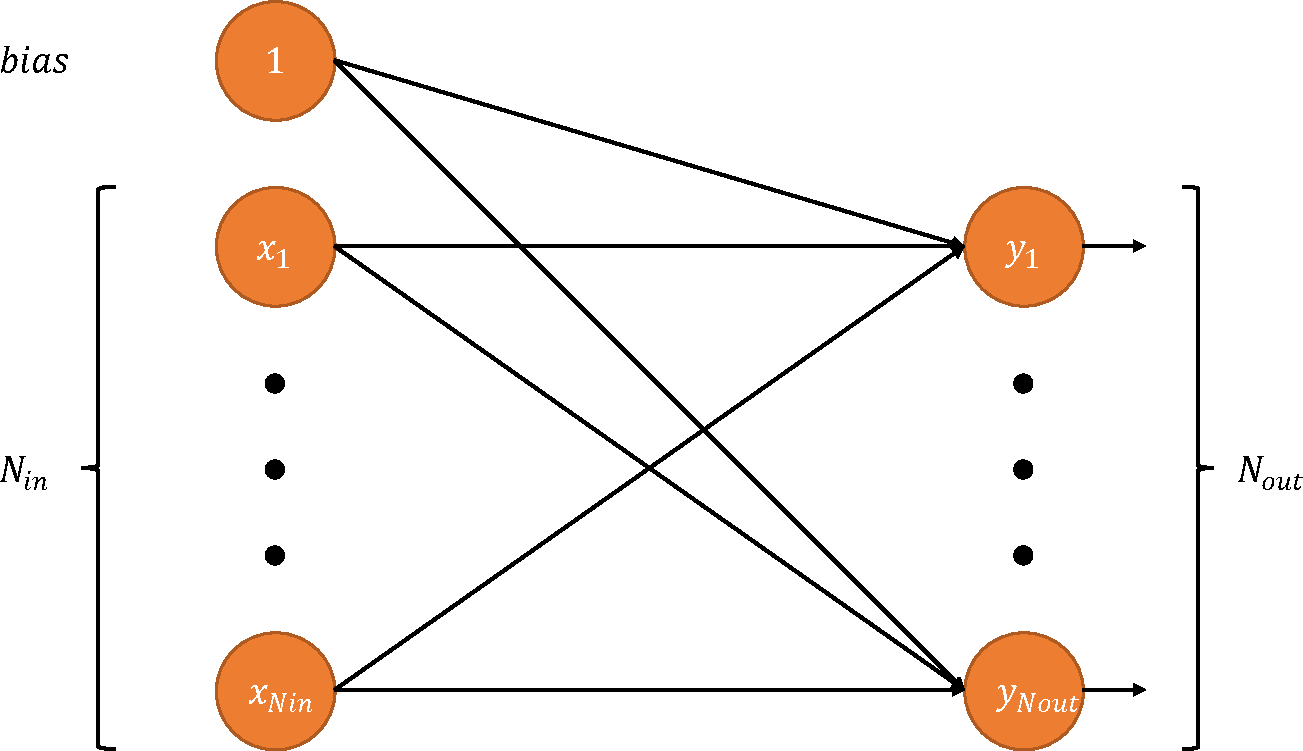
\includegraphics[width=\textwidth]{fcl.pdf}
    \caption{A fully connected layer}
    \label{fig:fcn}
\end{figure}

In the fully-connected layer, each neuron is connected to all the inputs or neurons of previous layers (as the name suggests). Usually, the fully-connected layers are placed at the end of the \acrshort{cnn}. It takes the extracted features from the previous layersas input, which are converted as a one-dimension output \acrshort{fm}. Afterwards, it makes a non-linear classification of them \cite{khan_survey_2020}.

A fully-connected layer is characterized by the number of neurons, activation functions, and the values of weights. The output vector $\boldsymbol{y}$ can be expressed using equation \eqref{eq:fcn}, where $\boldsymbol{x}$ is the vector of the input of the layer and $x_0 = 1$ is the bias;   $\boldsymbol{w}$ is the vector of all the weights of the layer ($w^i_*$ are the weights of the ith perceptron and $w^*_0$ are the biases); $h$ is the activation function of the layer.
%
\begin{equation}
    \boldsymbol{y} = h(\boldsymbol{w}^T \boldsymbol{x}) \Leftrightarrow \forall o \in \{ 1, ..., N_{out} \} : y_o = h(\sum^{N_{in}}_{i=0} w^o_i \cdot x_i)
    \label{eq:fcn}
\end{equation}
%
As we have seen that perceptrons can be used to construct non-linear classifier, we see in the next section \ref{subs:2dconv} the main operation in the \acrshort{cnn}: the \textbf{convolution}, which extracts the feature from input images.

%
\subsection{Convolution layer} \label{subs:2dconv}
In a \acrshort{cnn}, the \textbf{convolutional layer} carries out the feature extraction process of the input image, also called the input \acrfull{fm}. It is the main operation in a \acrshort{cnn} and it is the layer that gives the network its name. The first layer extracts low-level features of the input \acrshort{fm} and the deepest layers use the low-level features to build high-level ones \cite{goodfellow_deep_2016}.

An input image is characterized by 3 parameters: \textbf{$N_{ix}$} the width, \textbf{$N_{iy}$} the height, and \textbf{$N_{if}$} the depth. We can illustrate then the input \acrshort{fm} as a cuboid composed of layers of pixels. An illustration is presented in figure \ref{fig:notation:ifm}.
The convolution layer correlates therefore input \acrshort{fm} and a 4D filter, to produce output \acrshort{fm}, which contains the high-level features \cite{zhao_towards_2018}. The output \acrshort{fm} is also characterized by its width $N_{ox}$, its height $N_{oy}$ and its depth $N_{of}$. We can also see a general output \acrshort{fm} in figure \ref{fig:notation:ofm}. As a result, the filter consists of $N_{of}$ kernels, where each kernel has size $N_{kx} \times N_{ky} \times N_{if}$, that we can see in figure \ref{fig:notation:k}).
%
\begin{figure}
    \centering
    %
    \begin{subfigure}{.32\textwidth}
    \centering
    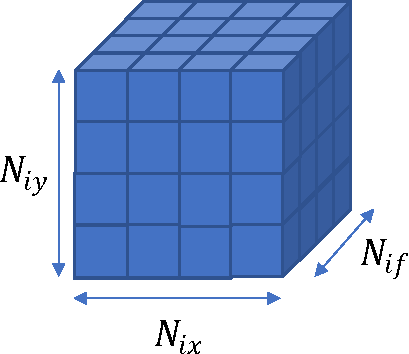
\includegraphics[width=\linewidth]{notifm.pdf}
    \caption{kernel-wise pruning}
    \label{fig:notation:ifm}
    \end{subfigure}
    %
    \begin{subfigure}{.32\textwidth}
    \centering
    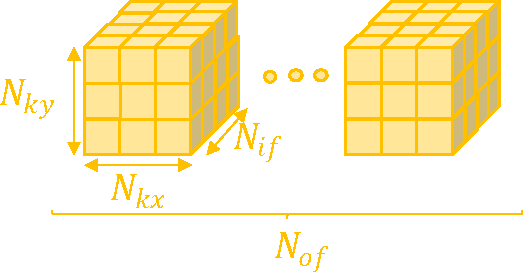
\includegraphics[width=\linewidth]{notk.pdf}
    \caption{Convolution kernel}
    \label{fig:notation:k}
    \end{subfigure}
    %
    \begin{subfigure}{.32\textwidth}
    \centering
    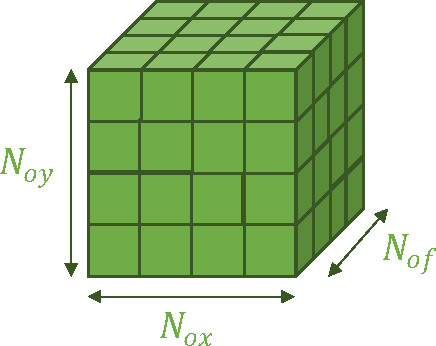
\includegraphics[width=\linewidth]{notofm.pdf}
    \caption{Output \acrshort{fm}s}
    \label{fig:notation:ofm}
    \end{subfigure}
    %
    \caption{Volumes involved in the convolution operations}
    \label{fig:notconv}
\end{figure}

Convolution is a specialized kind of linear operation. The convolution operation happens as follows. Each kernel acts like a sliding window on the input \acrshort{fm}. We extract a chunk of pixels of the same size of the kernel in the input \acrshort{fm} and perform an element-wise multiplication with the chunk of data and the kernel. We sum up the computed pixels to obtain one output pixel. Sliding this kernel on the input \acrshort{fm} will produce a channel of the output \acrshort{fm}, where the output pixel at position $(x, y)$ corresponds to the movement of the sliding window from the top left of the input \acrshort{fm}. Since one kernel produces one channel of the output \acrshort{fm}, having $N_{of}$ kernels produces then $N_{of}$ channels. An illustration of the convolution operation is in figure \ref{fig:convolution}.
%
\begin{figure}
    \centering
    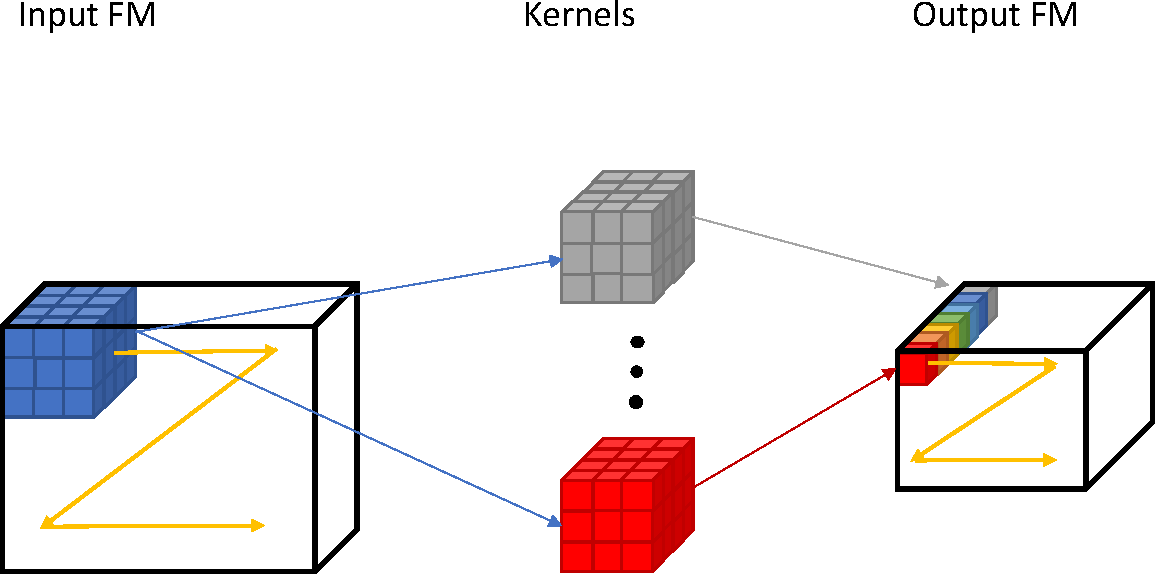
\includegraphics[width=\textwidth]{conv.pdf}
    \caption{Convolution operation}
    \label{fig:convolution}
\end{figure}

Except for $1 \times 1$ kernels, the sliding window can not cover all input pixels, and then there is a spatial reduction between the input and output \acrshort{fm}s, while there is an increase in the number of channel. However, we can keep the same dimensions using \textit{padding} on the boundary. It means that we pad the edges with extra pixels (usually of value 0).

Moreover, each time the sliding window performs a convolution, it shifts in the input \acrshort{fm}. The amount, by which the filter shifts, is called the \textit{stride} and it is initially set to 1. If we increase the stride, we can reduce the spatial dimensions of the output \acrshort{fm}. For example, if we use padding and a stride of 2, $\frac{N_{ix}}{N_{ox}} = \frac{N_{iy}}{N_{oy}} = \frac{1}{2}$, and the output \acrshort{fm} has 4 times fewer pixels. In section \ref{subs:pooling}, we introduce a new layer than can also reduce the spatial dimensions of the output \acrshort{fm}.

Finally, we can express the convolution operations mathematically as in equation \eqref{eq:conv}.
%
\begin{equation}
    \begin{split}
        \forall ox &\in \{ 1, ..., N_{ox} \}, oy \in \{ 1, ..., N_{oy} \}, of \in \{ 1, ..., N_{of} \} : \\
        FM_O[ox, oy, oc] &= \sum^{N_{if}}_{if=1}
        \sum^{N_{kx}}_{kx=1}
        \sum^{N_{ky}}_{ky=1}
        FM_I[ox \cdot S + kx - \lfloor \frac{N_{kx}}{2} \rfloor,  oy \cdot S + ky - \lfloor \frac{N_{ky}}{2} \rfloor, if] \cdot
        W^{of}_{if}[kx, ky]
    \end{split}
    \label{eq:conv}
\end{equation}

If we compare the convolutional layer with the fully-connected layer, the convolutional layer allows a sparse interaction (the kernel is smaller than the input), parameter sharing (we use the same parameter for more than one function) and equivariant representation (for some transformation, a change in the input reflects the same change in the output) \cite{goodfellow_deep_2016}. To illustrate weight sharing, in AlexNet \cite{krizhevsky_imagenet_2012}, 94\% of the weights are used in the fully-connected layers. But as said earlier, convolution is a computationally heavy operation. 90\% of the arithmetic operations are done in the convolutional layer.

As the convolution has a huge arithmetic complexity, we see in the following section \ref{subs:dsc} an alternate way to perform convolution to reduce this.

%
\subsubsection{Depthwise Separable Convolution}  \label{subs:dsc}
\acrfull{dsc} was first introduced by \textcite{sifre_ecole_2014}. According to \textcite{chollet_xception_2017}, \textquote{\textit{A depthwise separable convolution consists in a \textbf{depthwise convolution}, i.e. a spatial convolution performed independently over each channel of an input, followed by a \textbf{pointwise convolution}, i.e. a $1 \times 1$ convolution, projecting the channel's output by the depthwise convolution onto a new channel space}}.

It means that the \acrshort{dsc} is composed of a depthwise convolution followed by a pointwise convolution as illustrated in Figure \ref{fig:dsc}. This alternative form of convolution has been developed to reduce efficiently the arithmetic complexity, in exchange of a limited loss of accuracy \cite{liu_fpga-based_2019}. As a result, the \acrshort{dsc} has significantly fewer parameters and operations with respect to the standard convolution. Equations \eqref{eq:descopred} and \eqref{eq:descwgred} are used to calculate the reduction factors on weigths and on operations respectively, where $F_{*}$ are the factors of reduction, $W_{sc}$ and $O_{sc}$ are the weights and operations required for a standard convolution, and $W_{dsc}$ and $O_{dsc}$ are the weights and operations required for a \acrshort{dsc} \cite{liu_fpga-based_2019}.
%
\begin{equation}
    F_w = \frac{W_{dsc}}{W_{sc}} =
    \frac{N_{kx} \times N_{ky} \times N_{if} + N_{if} \times N_{of}}{N_{kx} \times N_{ky} \times N_{if} \times N_{of}} =
    \frac{1}{N_{of}} + \frac{1}{N_{kx} \times N_{ky}}
    \label{eq:descopred}
\end{equation}
\begin{equation}
    \begin{split}
        F_o &= \frac{O_{dsc}}{O_{sc}} = \frac{N_{kx} \times N_{ky} \times N_{if} \times N_{ox} \times N_{oy} + N_{if} \times N_{of} \times N_{ox} \times N_{oy}}{N_{kx} \times N_{ky} \times N_{if} \times N_{of} \times N_{ox} \times N_{oy}} \\
        &= \frac{1}{N_{of}} + \frac{1}{N_{kx} \times N_{ky}}
    \end{split}
    \label{eq:descwgred}
\end{equation}

Using equation \eqref{eq:descopred} and equation \eqref{eq:descwgred} and $3 \times 3$ kernels, the reduction of computation and parameters in comparison with the standard convolution is about 9 times \cite{zhang_channel_2019}.
%
\begin{figure}
    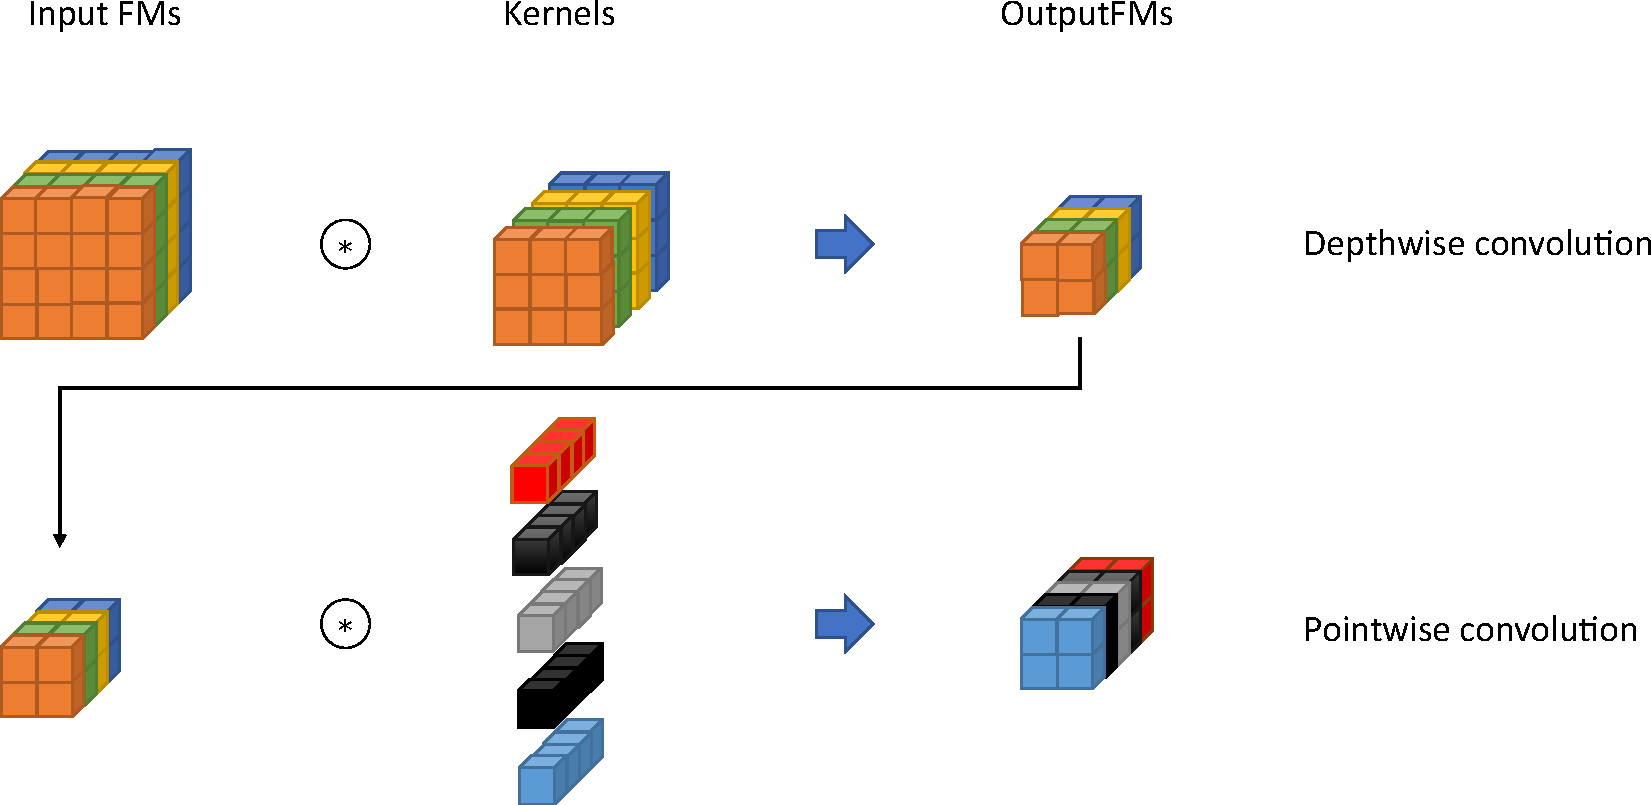
\includegraphics[width=\textwidth]{dsc.pdf}
    \caption{Depthwise Separable Convolution}
    \label{fig:dsc}
\end{figure}

%
\subsubsection{Pooling} \label{subs:pooling}
A Pooling layer is used to replace the output of the previous layer by a summary statistics of this output \cite{goodfellow_deep_2016}. They are usually inserted between the successive convolutional layer to modify the output further. Its goal is first to make the output approximately invariant to small translations and it also reduces the spatial size of each output \acrshort{fm}. It means that the memory needed to store the parameters is reduced \cite{goodfellow_deep_2016}. It also reduces the number of parameters and the computation of the network while also increasing the receptive field \cite{shawahna_fpga-based_2019}.

The pooling layer divides each \acrshort{fm} into regions of size $K \title K$ and outputs one pixel from each region. This way, is kept constant while their spatial size is reduced by $K$. Various pooling functions exist, but the most common form uses filters of size $2 \times 2$ where for example the MAX or AVG operation selects the highest pixel from 4 samples their average respectively (meaning a 75\% reduction of the pixels) \cite{suda_throughput-optimized_2016}. Figure \ref{fig:pool} illustrates an example of a pooling layer.
%
\begin{figure}
    \centering
    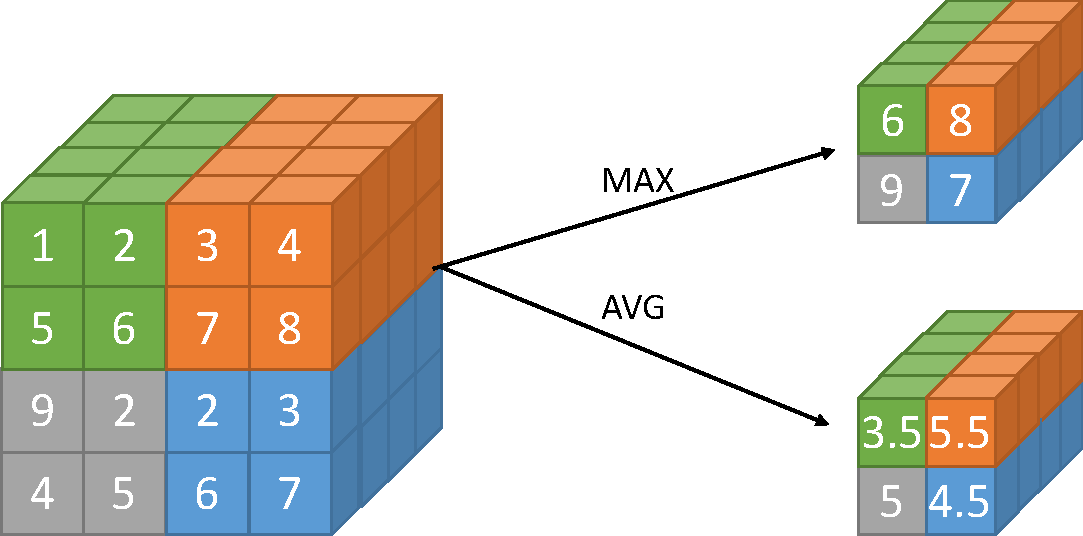
\includegraphics[width=0.8\textwidth]{pooling.pdf}
    \caption{An example of pooling layers}
    \label{fig:pool}
\end{figure}

%
\subsubsection{Summary}
%
The summary of this section is provided in Figure \ref{fig:layer:summary}. First, an input image is fed to the \acrshort{cnn}. Then, three different kinds of layers can be used:
%
\begin{enumerate}
    \item \textbf{The convolutional layer}, which extracts the features from the input.
    \item \textbf{The pooling layers}, which summarizes the output of the previous layer.
    \item \textbf{The fully connected layer}, which is a non-linear classifier.
\end{enumerate}
%
A typical \acrshort{cnn} is composed of two parts, which are built from stacking the previously mentioned layers \cite{matteucci_artificial_2019}:
\begin{enumerate}
    \item \textbf{The feature extractor} part, composed of blocks made of convolutional, activation, and pooling layers.
    \item \textbf{The classifier} part, composed only of fully connected layers.
\end{enumerate}
%
\begin{figure}[H]
    \centering
    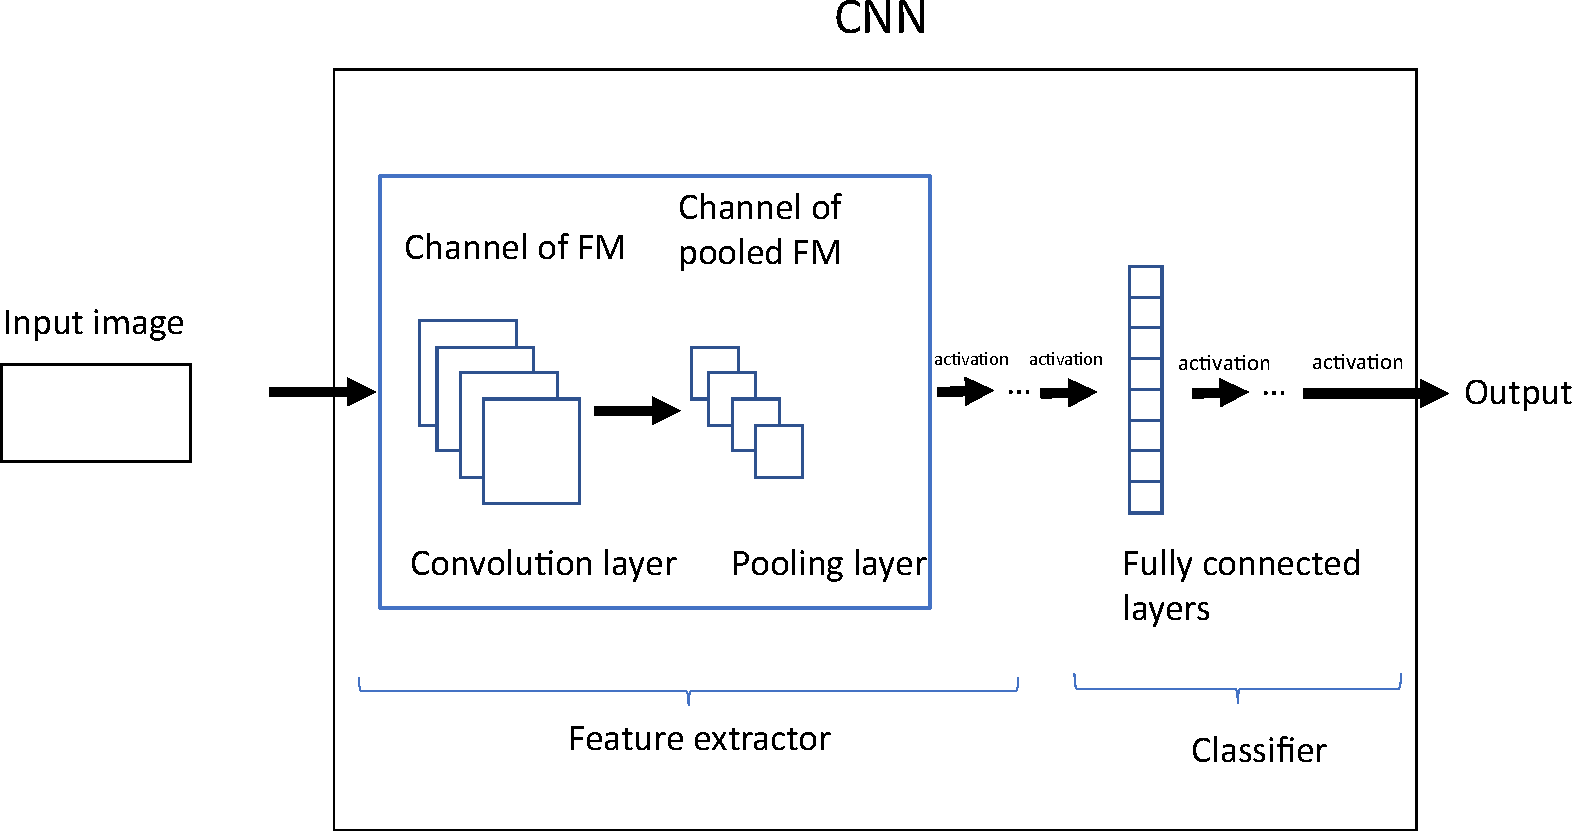
\includegraphics[width=0.75\textwidth]{cnn_summary.pdf}
    \caption{Working principle of a CNN and the different layers which composing it}
    \label{fig:layer:summary}
\end{figure}
%
\subsection{CNN Models} \label{subsec:models}
After the analysis of the CNN structure in Section \ref{subsec:layer}, this section details some of the well-known \acrshort{cnn} networks. They are examples of how to construct an efficient \acrshort{cnn}.

%
\subsubsection{AlexNet}
%
AlexNet is a famous \acrshort{cnn} which was developed in 2012 by \textcite{krizhevsky_imagenet_2012}. It is a breakthrough in the deep \acrshort{cnn} field and this model won the ImageNet competition. Krizhevsky et al. used some parameters optimizations and made the model deeper in order to considerably improve the learning ability of the CNN \cite{khan_survey_2020}. It is composed of 5 convolutional layers and 3 fully-connected layers, as seen in Figure \ref{fig:alexnet}. Each convolutional layer has a ReLU activation function and it uses pooling.
%
\begin{figure}[H]
    \centering
    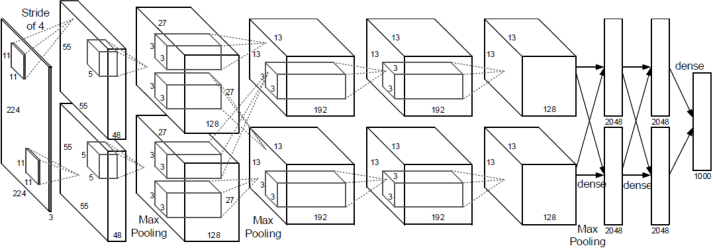
\includegraphics[width=\textwidth]{alexnet.pdf}
    \caption{An illustration of the architecture of AlexNet \cite{krizhevsky_imagenet_2012}}
    \label{fig:alexnet}
\end{figure}
%
\subsubsection{VGG}
%
After the success of AlexNet in 2012, research was made to reduce the computational complexity while keeping the accuracy. In 2014, VGG, a deeper variant of AlexNet was developed by \textcite{simonyan_very_2015}. It is composed of 5 groups of convolutional layers, where the number of layers depends on the version of VGG. It won the localization in the ImageNet challenge in 2014 \cite{simonyan_very_2015}. An illustration is provided by Figure \ref{fig:vgg}. This level of depth was possible thanks to the application of very small ($3 \times 3$) convolution kernels. They allow a larger receptive field with fewer parameters and more non-linearities than a larger kernel. However, it has a high memory request. 100MB per image needs to be stored in all \acrshort{fm}s for the forward propagation \cite{matteucci_artificial_2019}.
%
\begin{figure}[H]
    \centering
    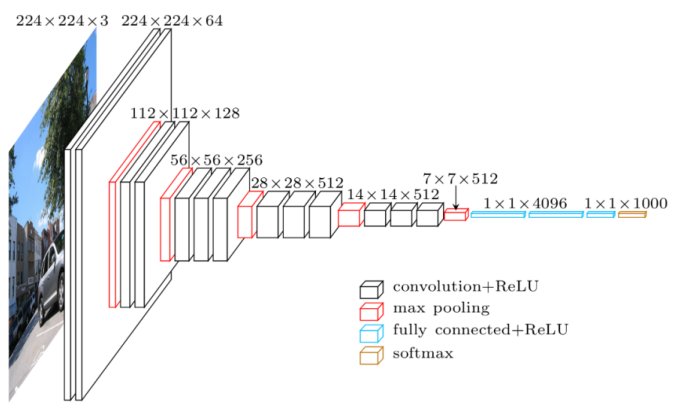
\includegraphics[width=0.75\textwidth]{VGG.pdf}
    \caption{An illustration of the architecture of VGG16 \cite{simonyan_very_2015}}
    \label{fig:vgg}
\end{figure}
%
\subsubsection{ResNet}
%
\textcite{he_deep_2016} developed ResNet in 2015. It is a very deep network which can contain from 50 to 1000 convolutional layers. It is composed of structures which are more complex and irregular than in the networks described previously. \textcite{he_deep_2016} showed that an increase of the depth of the network does not leads to an improvement of the performance. Indeed, beyond a certain amount of layers, a continuous increase of the depth leads to the degradation of the accuracy. This is not due to overfitting. It is because the deeper models are harder to optimize than shallower ones (vanishing gradient described in Section \ref{subs:trainbackward}) \cite{matteucci_artificial_2019}. 

However, deeper networks should at least have similar or better performance than shallower ones. Indeed, let’s compare a deeper and a shallower network. If the deeper network is composed of the same layers than the shallower one and that the other added layers are just identity mapping, then the network should have the same performance than the shallower one. Therefore, a deeper network should not have worse performance than shallower ones \cite{matteucci_artificial_2019}.

To overcome this issue, \textcite{he_deep_2016} introduced an \textit{identity shortcut connection} which skips one or more layers and set weights to the identity, as can be seen in Figure \ref{fig:resnet}. These weights associated to the shortcut connection can be used to learn a residual $\mathcal{F}(x)$ in order to improve the solution. The performance of this very deep network allowed it to win the 2015 ILSVR for both localization and classification.
%
\begin{figure}[H]
    \centering
    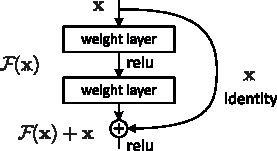
\includegraphics[width=0.7\textwidth]{resnet.pdf}
    \caption{ResNet building block, from \cite{he_deep_2016}}
    \label{fig:resnet}
\end{figure}
%
\subsubsection{MobileNetV2} \label{subs:mbv2}
%
According to \textcite{cheng_recent_2018}, the performance of \acrshort{cnn} in recent years became outstanding. These improvements came at the cost of storage and computational complexity. It is not an issue for the \acrshort{cnn} training phase, because the GPU and CPU also gained in computational units and memory. However, for the inference phase, the computational complexity and the storage requirements are way beyond the capabilities of most of the embedded applications and mobile devices such \acrshort{fpga} \cite{cheng_recent_2018}.
%
\begin{itemize}
    \item The enormous computational complexity of \acrshort{cnn}s makes it difficult to deploy on real-time applications and it consumes battery power.
    \item The large number of parameters of \acrshort{cnn}s consumes considerable storage and run-time memory.
\end{itemize}

In order to overcome this issue, \textcite{sandler_mobilenetv2_2018} introduced a network called MobileNetV2 in 2018. It is specifically developed for constrained environments. First, the size and number of operations is decreased thanks to DSC (see Section \ref{subs:dsc}) and thanks to a new type of layer \textit{inverted residual with a linear bottleneck}, which can be observed in Figure \ref{fig:invreslinbot} and Table \ref{tab:invreslinbot}.
This layer is composed of a $1 \times 1$ convolution to expand the number of the input \acrshort{fm} channels by a factor $t$ ($N_{intf} = t \times N_{if}$). It is then followed by a \acrshort{dsc}. The purpose of the first convolution layer which increases the number of channels is supposed to counterbalance the loss of information that occurred by the ReLU activation. They also added a skip connection to build a network of great depth, and the last convolution has a linear activation function \cite{sandler_mobilenetv2_2018}.
%
\begin{figure}[H]
    \centering
    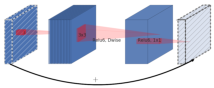
\includegraphics[width=\textwidth]{mbnv2.pdf}
    \caption{inverted residual with linear bottleneck \cite{sandler_mobilenetv2_2018}}
    \label{fig:invreslinbot}
\end{figure}
%
\begin{table}
    \center
    \begin{tabular}{c|c|c}
        Input & Operetor & Output \\
        \hline \hline
        $N_{ix} \times N_{iy} \times N_{if}$ & $1 \times 1$ conv2d, ReLU6 & $N_{ix} \times N_{iy} \times (t \times N_{if})$ \\
        $N_{ix} \times N_{iy} \times (t \times N_{if})$ & $3 \times3$ dwise s=$s$, ReLU6 & $\frac{N_{ix}}{s} \times \frac{N_{iy}}{s} \times (t \times N_{if})$ \\
        $\frac{N_{ix}}{s} \times \frac{N_{iy}}{s} \times (t \times N_{if})$ & $1 \times 1$ conv2d & $\frac{N_{ix}}{s} \times \frac{N_{iy}}{s} \times N_{of}$ \\
        \hline \hline
    \end{tabular}
    \caption{inverted residual with linear bottleneck \cite{sandler_mobilenetv2_2018}}
    \label{tab:invreslinbot}
\end{table}

More information about the structure of MobileNetV2 can be found in Appendix \ref{appendix:mbv2}.

%
%
\subsection{Training} \label{subsec:train}
The previous section described the common building blocks present in \acrshort{cnn}s and how to design a \acrshort{cnn}. This section aims at detailing how a network improves automatically its performance for a specific task. This is called \textit{learning}.

The learning phase starts after designing the network. However, before the model can learn, we have to initialize the weights. The most common initialization is a random Gaussian distribution \cite{he_delving_2015}. However, the learning phase is affected by the initial values of the weights. If it is too small the network does not learn or if it is too large it might take a very long time to converge. Different initializations were suggested to improve the learning phase: Xavier initialization \cite{glorot_understanding_2010} and He initialization \cite{he_delving_2015}.

When values are assigned to the weights, the back-propagation algorithm can be performed to improve the efficiency of the network. The back-propagation algorithm is composed of two steps: the forward-propagation and the back-propagation. In the following sections, we briefly review each of them.
%
\subsubsection{Forward-propagation} \label{subs:trainforward}
%
The first step of the backpropagation algorithm is the forward propagation. During this step, the training data are used as input of the model and each input is propagated through the network using the initialized weights. A vector of outputs is produced and is compared using a loss function (for example mean-square error defined by Equation \eqref{eq:mse}) with the label of the input (target $\boldsymbol{t}$) \cite{matteucci_artificial_2019}. The weights are then adjusted in order minimize the loss function. This can be done using the algorithms found in the next section. When the model is trained, the inference consists only of the forward propagation \cite{abdelouahab_accelerating_2018}.
%
\begin{equation}
    L(\boldsymbol{x}, \boldsymbol{w}) = \sum^{N}_{i=1} (t_i - p(x_i, \boldsymbol{w}))^2
    \label{eq:mse}
\end{equation}

%
\subsection{Back-propagation} \label{subs:trainbackward}
According to \textcite{ruder_overview_2017}, gradient descent optimization algorithms are the most popular to perform optimizations on \acrshort{nn}. These algorithms derive from the idea of gradient descent. As said in the previous section, gradient descent is a way to minimize the loss function, parametrized by the model's parameters (weight). We can, therefore, describe gradient descent algorithm using equation \eqref{eq:gd}, where $\eta$ is the learning rate, a positive scalar determining the size of the step in the direction minimizing the gradient \cite{goodfellow_deep_2016}. If we update the weight in the opposite direction of the gradient, we can reach a local minimum.
%
\begin{equation}
    \boldsymbol{w} = \boldsymbol{w} - \eta \frac{ \partial L( \boldsymbol{x}, \boldsymbol{w} ) }{\partial \boldsymbol{w}}
    \label{eq:gd}
\end{equation}

\textbf{The original gradient descent} or \textbf{batch gradient descent }computes the gradient using the whole dataset (the batch). We see how to compute the gradient on equation \eqref{eq:gd-grad}. This might be impossible to do in practice if the dataset is too large. Variations have then be proposed to make the gradient descent to be practical.
%
\begin{equation}
    \frac{ \partial L( \boldsymbol{x}, \boldsymbol{w} ) }{\partial \boldsymbol{w}} = \frac{1}{Nin} \sum^{Nin}_{i = 0} \frac{ \partial L( x_i, \boldsymbol{w} ) }{\partial \boldsymbol{w}}
    \label{eq:gd-grad}
\end{equation}

\textbf{Stochastic gradient descent}, instead of using the entire dataset, performs the gradient descent algorithm on one sample at a time. We see how to compute the gradient on equation \eqref{eq:sgd-grad}. It avoids the redundant computation of the batch gradient descent. It learns faster and can reach better local minima, however, it is complicated to find the global minimum.
%
\begin{equation}
    \frac{ \partial L( \boldsymbol{x}, \boldsymbol{w} ) }{\partial \boldsymbol{w}} = \frac{ \partial L( x_i, \boldsymbol{w} ) }{\partial \boldsymbol{w}}
    \label{eq:sgd-grad}
\end{equation}

\textbf{Mini-batch gradient descent} is a trade-off between the two approaches. It performs an update of the weight for every mini-batch of $N$ training examples. It has better convergence  by reducing the variance and has less computation than batch gradient descent.
%
\begin{equation}
    \frac{ \partial L( \boldsymbol{x}, \boldsymbol{w} ) }{\partial \boldsymbol{w}} = \frac{1}{N} \sum^{N < Nin}_{i = 0} \frac{ \partial L( x_i, \boldsymbol{w} ) }{\partial \boldsymbol{w}}
    \label{eq:bgd-grad}
\end{equation}

%
%

% FPGA
\chapter{FPGA}
\label{chap:fpga}
\section{Loop optimization techniques} \label{sec:loopopti}
\acrfull{simd} accelerators were proposed to solve the static systolic array inefficiency. The general computation flow can be described as follow:
\begin{enumerate}
    \item Fetch \acrshort{fm}s and weights from the external memory (\acrshort{dram}) to on-chip buffer.
    \item The \acrshort{fm}s and weights are streamed into the \acrshort{pe}.
    \item
\end{enumerate}

%
\begin{tcolorbox}
    \textbf{Conclusions about the Background}:

    We have seen in this chapter what is a \acrshort{cnn}, how to build, and train it. We have also seen that the most performing models have a huge computational complexity and memory utilization, which limit the implementation of such models on mobile platforms, such as \acrshort{fpga}. We have also seen what is an \acrshort{fpga}, what are its components and how to construct an hardware design on it.
\end{tcolorbox}
% 
\afterpage{\blankpage}
\cleardoublepage
\newpage
